%%%%%%%%%%%%%%%%%%%%%%%%%%%%%%%%%%%
%%  Datenbank
%%%%%%%%%%%%%%%%%%%%%%%%%%%%%%%%%%%
\section{Analyse back end}
Der Kombi-Wettert-Transmitter sendet seine Daten über eine RS-484 Schnittstelle. Die Software \textit{WeatherDisplay} verarbeitet diese Daten und erstellt unterschiedliche Text-Files, die anschliessend von anderen Anwendungen, wie zum Beispiel \textit{WeatherDisplay Live}, verwendet werden. Zusätzlich sendet \textit{WeatherDisplay} einmal pro Minute sämtliche Werte an die MySQL-Datenbank. Abbildung \ref{img:datenfluss} zeigt den Datenfluss vom Sensor bis zur Webseite. 

\begin{figure}[h!]
	\centering
	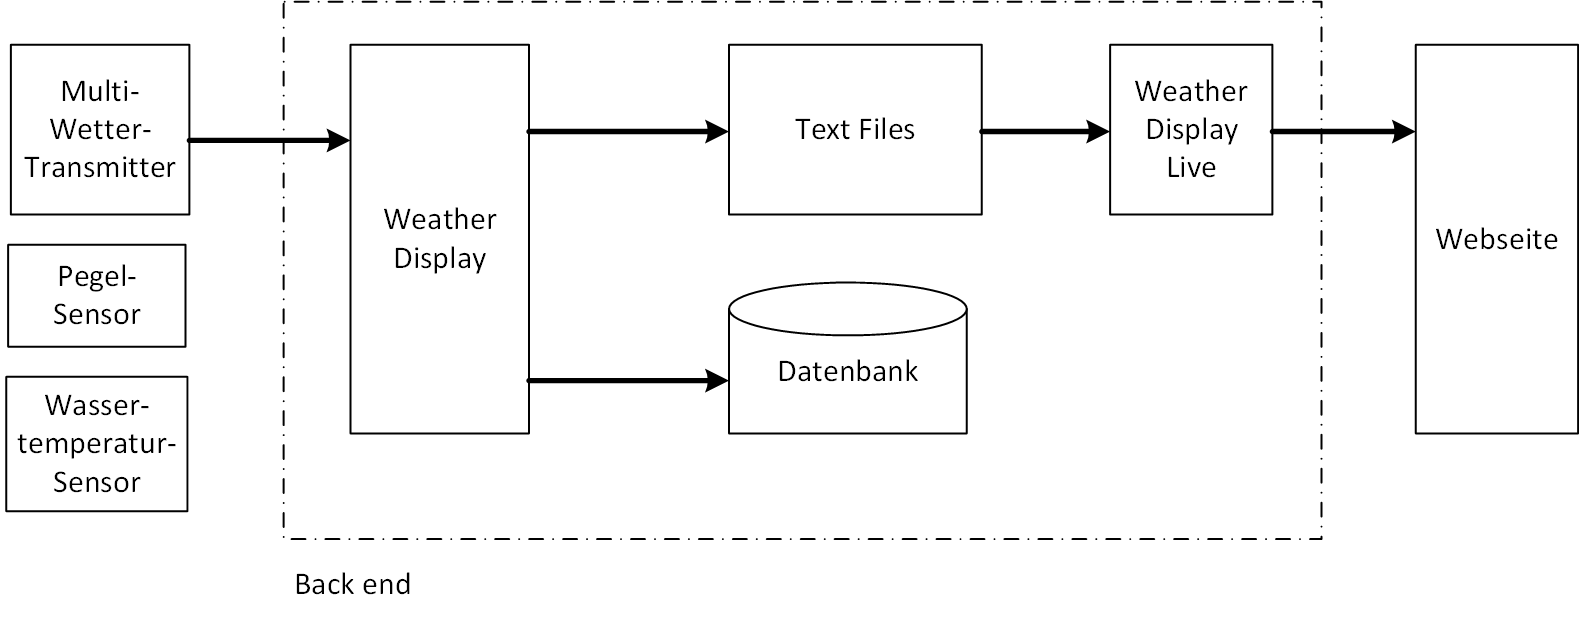
\includegraphics[width=1\linewidth]{img/datenfluss.pdf}
	\caption{Datenfluss vom Sensor bis zur Webseite}
	\label{img:datenfluss}
\end{figure}



% ################################
% Schnittstelle zum Kombi-Wetter-Transmitter
% ################################
\subsection{Schnittstelle zum Kombi-Wetter-Transmitter}
Die Software \textit{WeatherDisplay} \footnote{ \url{http://www.weather-display.com}} dient als Schnittstelle zum Kombi-Wetter-Transmitter. Der Auftraggeber möchte diese Software beibehalten. Interessant für uns sind deshalb die Daten, die  \textit{WeatherDisplay} liefert. Dies sind vier verschiedene Text-files, deren Inhalt in Tabelle~\ref{table:text-files} aufgelistet sind, sowie ein minütlicher Eintrag sämtlicher Messwerte in die Datenbank.
\newline

\begin{table}[h]
\centering
\begin{tabular}{|l|l|l|l|l|}
\hline
 Name			&  Anzahl Daten	& 	Zeitspanne  		& 	Intervall			\\ \hline
 Clientraw.txt 		&  174			&  	10min/20h zurück 	& 	5 Sekunden 		\\ \hline
 Clientrawextra.txt	&  767 			&  	24h zurück 		& 	1 Stunde 			\\ \hline
 Clientrawdaily.txt 	&  442 			&  	30 Tage zurück 	&  	1 Tag 			\\ \hline
 Clientrawhour.txt	&  673			&  	1h zurück 			& 	1 Minute 			\\ \hline
\end{tabular}
\caption{Von \textit{WeatherDisplay} erstellte Text-Files}
\label{table:text-files}
\end{table}

\noindent
%\subsection*{Problem}
Der Nachteil ist, dass der Inhalt und Aufbau der Text-Dateien fix vorgegeben sind. Das bedeutet insbesondere, dass das Intervall der Messresultate nicht verändert werden kann. Bei einem 24-Stunden-Rückblick beispielsweise ist nur jeweils ein Wert pro Stunde vorhanden, was zu einer sehr groben Darstellung führt, wie in Abbildung~\ref{img:wind-richtung}, links erkennbar. Zudem sind in diesen Text-Files nur die Daten des Kombi-Wetter-Transmitters aufgeführt. Weitere Sensoren wie Pegel und Wassertemperatur sind nicht enthalten. Diese müssen ohnehin separat behandelt werden.
\newline

\noindent
%\subsection*{Lösungsansatz}
Während der Bachelor-Arbeit soll geprüft werden, in wie weit die Daten aus den Text-Files für die Erstellung der neuen Anzeige-Elemente verwendet werden können. Die Alternative besteht darin, sämtliche Daten aus der Datenbank zu beziehen.


% ################################
% Speicherung historischer Daten
% ################################
\subsection{Speicherung historischer Daten}
Um die Daten der Wetterstation zu speichern, wird eine MySQL-Datenbank verwendet. Da die Wetterstation kontinuierlich umgebaut und erweitert wurde, besteht die Datenbank aus mehreren Tabellen, die sich in Inhalt, Intervall und Zeitraum unterscheiden, wie in Tabelle~\ref{table:db-tables} dargestellt. Bisher wurden diese Daten nicht verwendet. Es ist aber vorgesehen, dass es zukünftig auf der Webseite eine Möglichkeit gibt, auf die historischen Daten zuzugreifen.
\newline

\begin{table}[h!]
\resizebox{\textwidth}{!}{%
\begin{tabular}{|l|l|l|l|l|}
\hline
 Tabelle		&  Inhalt								& 	von  			& 	bis 			& 	Intervall\\ \hline
 tblgestern 	&  min und max Werte					&  	25.02.2005 	& 	14.07.2012 	& 	24h \\ \hline
 tblwellen		&  Pegel, Wellenhöhe, und Wassertemperatur 	&  	29.10.2013 	& 	28.01.2014  	& 	10min \\ \hline
 tblwind 		&  Windgeschwindigkeit- und Windrichtung 	&  	29.10.2013 	& 	28.01.2014 	&  	1min \\ \hline
 wx-data 		&  alle vom KWT gemessenen Werte		&  	25.02.2015 	&	heute  		& 	1min \\ \hline
 wx-pegel  	&  \multicolumn{4}{l|}{enthält keine Daten, da der Pegelsensor defekt ist} \\ \hline
\end{tabular}%
}
\caption{Vorhandene Daten in der Datenbank}
\label{table:db-tables}
\end{table}

\noindent
%\subsection*{Problem}
Um auf die Daten zugreifen zu können, müssen mehrere Tabellen abgefragt werden, was die Query und die Anzeige der Daten erschwert. Zudem fehlt ein Konzept, welche Daten wo, wie und wie häufig gespeichert werden sollen.
\newline

\noindent
%\subsection*{Lösungsansatz}
Während der Bachelor-Arbeit soll deshalb ein Konzept erarbeitet und umgesetzt werden, damit die historischen Daten auf der Webseite der Wetterstation Arbon abgefragt und dargestellt werden können.


% ################################
% Datenmanagement
% ################################
\subsection{Datenmanagement}
Täglich fallen alleine vom Kombi-Wetter-Transmitter 1440~Datenbank-Einträge an. Das sind rund eine halbe Million Einträge pro Jahr. Diese Daten werden seit 2015 gespeichert und nicht ausgedünnt. Zur Zeit benötigt die Datenbank etwa 320~MB Speicherplatz.
\newline

\noindent
%\subsection*{Problem}
Der Speicherplatzbedarf der Datenbank ist momentan noch kein Problem. Hingegen ist davon auszugehen, dass die Abfragegeschwindigkeit und die Datenmenge der Antwort bei so vielen Datensätzen Probleme bereiten wird.
\newline

\noindent
%\subsection*{Lösungsansatz}
Die Daten sollen deshalb zeitabhängig ausgedünnt werden. Die Zeitabstände, in denen die Daten gelöscht, beziehungsweise gemittelt werden, müssen während der Bachelor-Arbeit mit dem Auftraggeber abgesprochen werden. Weiter soll geprüft werden, ob zusätzliche Tabellen mit zum Beispiel den Minimal- und Maximalwerten erstellt werden sollen, um die Performance der Abfragen zu erhöhen.


